\section{Question 3}

\begin{question}
    Using the \textit{chredlin} data from the faraway package in R, fit a linear model of \textit{theft} against \textit{age}. Further, fit a linear model of \textit{theft} against \textit{age} and $\textit{{age}}^2$. Plot both models over the scatter plot of \textit{theft} against \textit{age}. Which model seems to be a better fit?
\end{question}

\begin{answer}
    I used the following codes fitting the model $1$ of the \textit{theft} against \textit{age}:
    \begin{verbatim}
        library(faraway)
        # Fit the model of theft against age
        lm1 <- lm(chredlin$theft~chredlin$age)
        # Show the result
        lm1
    \end{verbatim}
    Then, I get the result of the model which is $\widehat{theft} = 13.4408 + 0.3136 \cdot age$.
    
    I used the codes below fitting the model $2$ of the \textit{theft} against \textit{age} and \textit{age${}^2$}
    \begin{verbatim}
        # Fit the model of theft against age and age^2
        lm2 <- lm(chredlin$theft~chredlin$age + I(chredlin$age^2))
        # Show the result
        lm2
    \end{verbatim}
    I get the model $2$ which is $\widehat{theft} = 6.247810 + 0.698292 \cdot age - 0.003869 \cdot {age}^2$.
    \begin{verbatim}
        plot(chredlin$theft~chredlin$age, xlab = "age", ylab = "theft")
        # Plot the model 1
        abline(lm1)
        # Plot the model 2
        points(chredlin$age, lm2$fitted, type = "l", col = "blue")
    \end{verbatim}
    By the codes above, I made a scatter plot of \textit{theft} against \textit{age} with both models fitted, and I used color blue to indicate the model $2$, while the model $1$ is shown in black. I have the following figure.
    \begin{figure}[H]
        \centering
        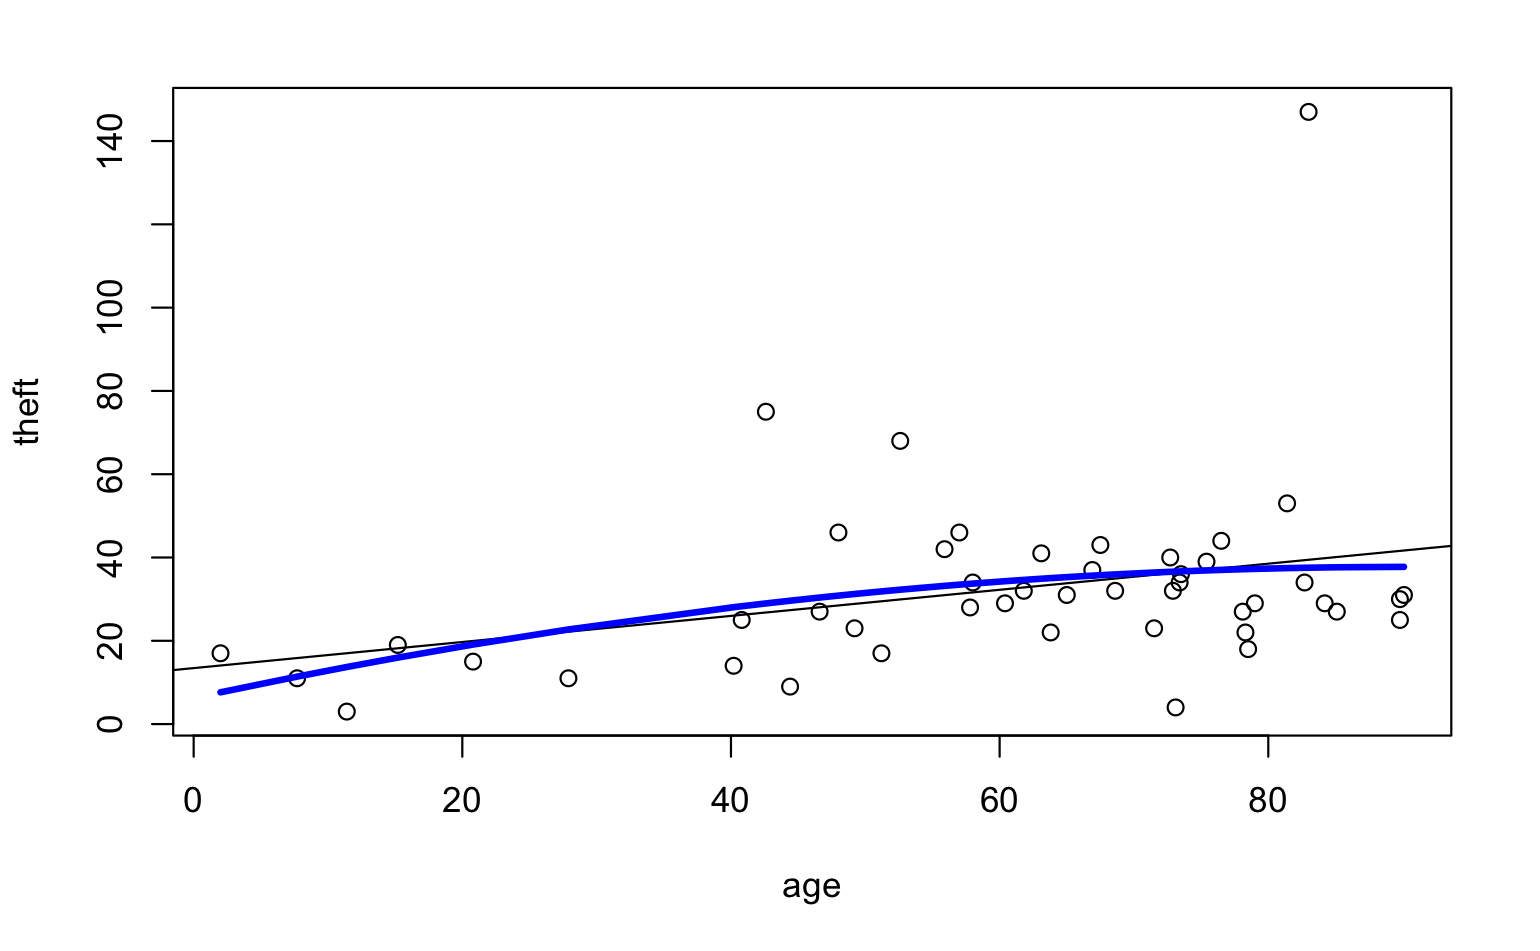
\includegraphics[width=0.8\textwidth]{Figure 3.png}
        \caption{\label{fig:fig3}plot of \textit{theft} against \textit{age} with fitted models}
    \end{figure}
    From the Figure \ref{fig:fig3}, we can tell that the model $1$ seems to be a better fit, since it tells the trend of the data, while the second model is too complicated and is overfitted.
\end{answer}
